\textbf{\hl{IS THIS SECTION NECESSARY?}}

\subsection{General Idea}

Figure \ref{fig.diffTraceOverview} shows a general overview of DiffTrace and its components.

\begin{figure}[t]
\caption{diffTrace Overview}
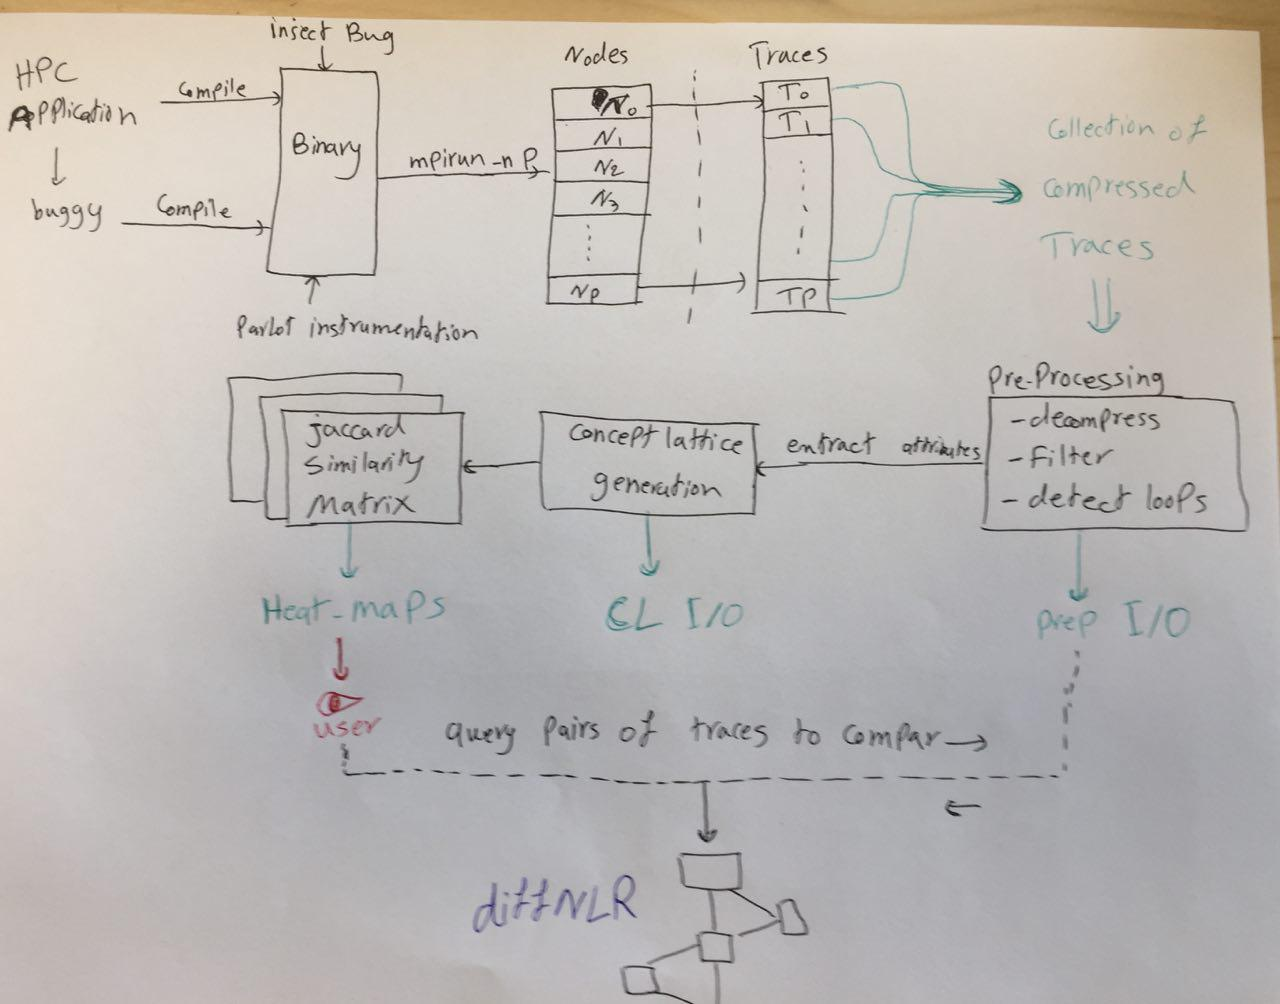
\includegraphics[width=0.45\textwidth]{overviewSketch.jpg}
\label{fig.diffTraceOverview}
\end{figure}


\subsection{Fault Injection??}
\subsection{ParLOT}
How we collect ParLOT traces? Is that necessary?
\subsection{Filter}
Include a table with all filters and their regular expressions
\subsubsection{General Filters}
\begin{itemize}
\item Returns
\item .plt
\item Memory
\item Network
\item Polling
\item String
\item Customize
\item IncludeEverything
\end{itemize}
\subsubsection{Target Filters}
\begin{itemize}
\item MPI\_
\item MPIall
\item MPI\_ Collectives
\item MPI\_ Send/Recv
\item OMPall
\item OMPcritical
\item OMPmutex
\end{itemize}

\subsection{Nested Loop Recognition}
\subsubsection{Background}
\subsubsection{Implementation}


\subsection{Concept Lattice Analysis}
\subsubsection{Background}
\begin{itemize}
\item FCA (formal concept analysis) background and citations
\item FCA applications in all areas
\item FCA applications in Data Mining and Information Retrieval
\item FCA applications in distributed systems (Garg's work)
\item intro to Concept, Object, Attribute and other definitions
\end{itemize}

\subsubsection{Objects/Attributes}


Mapping of Object/Attribute (general) to Trace/Attribute (clTrace)

What do we expect to gain by doing so
\begin{itemize}
\item Single entity represents the whole execution of HPC application (can be used as signature/model in ML)
\item Classifying similar behavior objects(traces)
\item Efficient Incremental CL building makes it scalable 
\item Efficient full pair-wise Jaccard Similarity Matrix extraction 
\end{itemize}
\subsubsection{CL generation}

\begin{itemize}
\item background
\item current approach
\end{itemize}

\subsubsection{Jaccard Similarity Matrix}

\begin{itemize}
\item background
\item LCA
\item Benefits
\end{itemize}


\subsection{diffNLR}
\begin{itemize}
\item motivation
\item diff algorithm
\item visualization
\end{itemize}

\subsection{FP-Trace}
